\section{HLASM context tables}

HLASM context tables (in code referred simply as hlasm context) is composition of tables and stacks that describe state of the currently processed open-code (see \cref{fig06:hlasm}). The object is persistent between source files within an open-code. It is created in analyzer and has the same lifespan. 

\begin{figure}
	\centering
	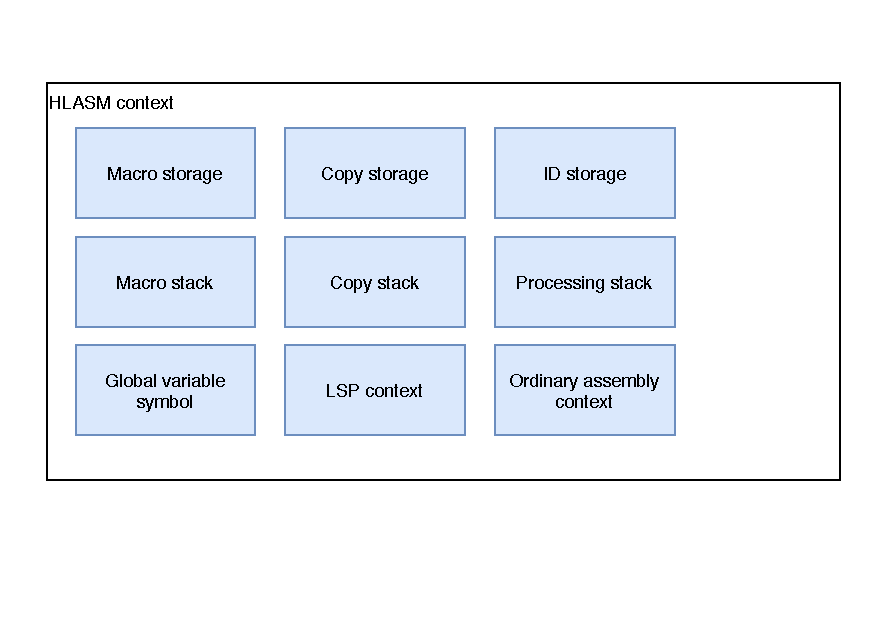
\includegraphics[width=\textwidth / 2]{img/hlasm_arch}
	\caption{The composition of HLASM context tables component}
	\label{fig06:hlasm}
\end{figure}

\subsection{Macros}

HLASM context stores visited macro definitions located in the \emph{macro strorage}. 

Macro definition is represented by:
\begin{enumerate}
	\item \emph{Macro name} --- to identify the macro.
	\item \emph{Calling parameters}. They are assigned real parameters when the macro is called.
	\item \emph{Block of statement}. Represents the body of the macro.
	\item \emph{Block of copy nestings}. It is array with one-to-one relation with block of statements. Each entry is a list of in-file locations that represents how much was the statement nested in COPY calls.
	\item \emph{Label storage}. The storage of sequence symbol that occur in the macro definition.
\end{enumerate}

When macro is called, \emph{macro invocation} object is created. It shares the content of a respective macro definition with an exception of calling parameters as they are assigned real value passed with the call. Also, it contains information which is the current statement in the invocation.

The macro invocation is stored in the context's \emph{scope stack}.

\subsection{Scope stack}

This stack holds information about the scope of variable symbols (see ??). The scope changes when macro is visited and the initial scope is the open-code. 
The stack contains:
\begin{itemize}
	\item In-scope variable symbols.
	\item In-scope sequence symbols.
	\item Pointer to the macro invocation (NULL if in open-code).
	\item Branch counter (for ACTR instruction).
\end{itemize}

\subsection{COPY}

HLASM context stores visited COPY members in the \emph{copy strorage}.

COPY member definition is much simpler as it does not hold any more semantic information than a peace of string.

When copy is visited, copy member invocation is created and pushed in the copy stack of last entry of the \emph{source stack}.

\subsection{Source stack and Processing stack}

This stacks are responsible for the nests of opened files (source stack) and what they are opened for (processing stack). As the relation of source entry and processing entry is one-to-many, the information is stored in two arrays rather than one.

When an statement processor (see \cref{sect_proc}) change (e.g. macro or copy definition is processed, lookahead is needed, ...), this information is stored in the processing stack. When, during the change, new file is opened then source stack is updated correspondingly.

Source stack contains copy stack active for a respective source file and data that locates last processed statement in the source file.
Processing stack contains \emph{processing kind}.

The reasoning of organizing this two stacks in such a way is:
\begin{enumerate}
	\item Context has enough information to fully reconstruct the statement.
	\item Easy retrieval of the correct copy stack for copy statement provider.
\end{enumerate} 

\subsection{ID storage}

ID storage holds the string identifiers that are used by the open-code. 
It stores the string and retrieves a pointer. It is guaranteed that if two different strings with the same value are passed to the storage, the resulting pointers are equal.

It simplifies work with IDs and saves space. 

\subsection{LSP context}

\subsection{Ordinary assembly context}

The above described structures aimed the high-level part of the language (code generation). As we move closer to the resulting object code of the source file, the describing structures get complicated. Therefore, HLASM context contains object storing just this part of the processing.

\begin{figure}
	\centering
	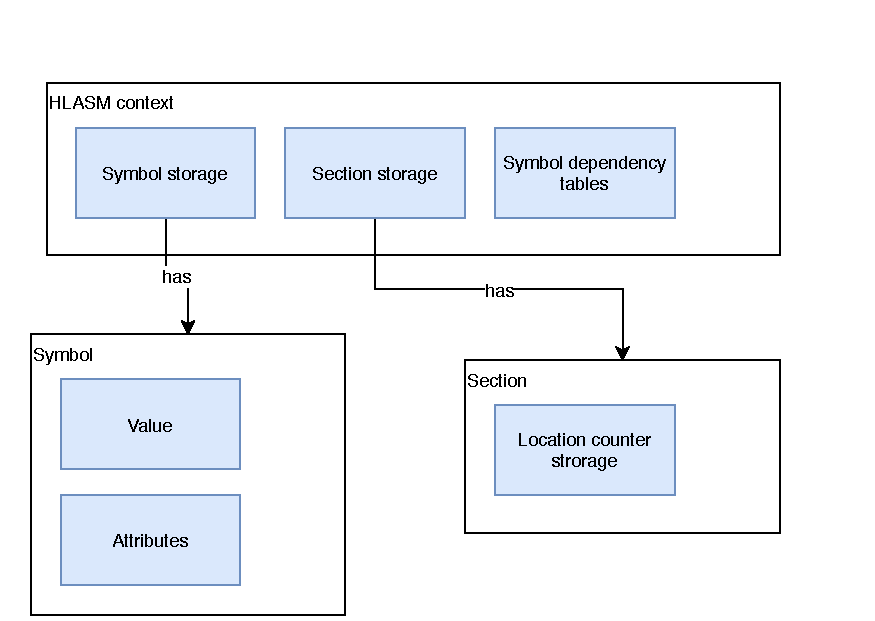
\includegraphics[width=\textwidth / 2]{img/ord_ctx_arch}
	\caption{The composition of Ordinary assembly context}
	\label{fig06:ord_ctx}
\end{figure}

Ordinary assembly context consists of three main components (see \cref{fig06:ord_ctx}):
\begin{enumerate}
	\item \emph{Symbol storage}. Stores ordinary symbols (see ??).
	\item \emph{Section storage}. Has notion of all generated sections, each section containing its location counter.
	\item \emph{Symbol dependency tables}. Contains yet unresolved dependencies between symbols prior to the currently processed instruction.
\end{enumerate}

